\section{Results \label{sec:results}}

\begin{figure*}[!b]
\centering
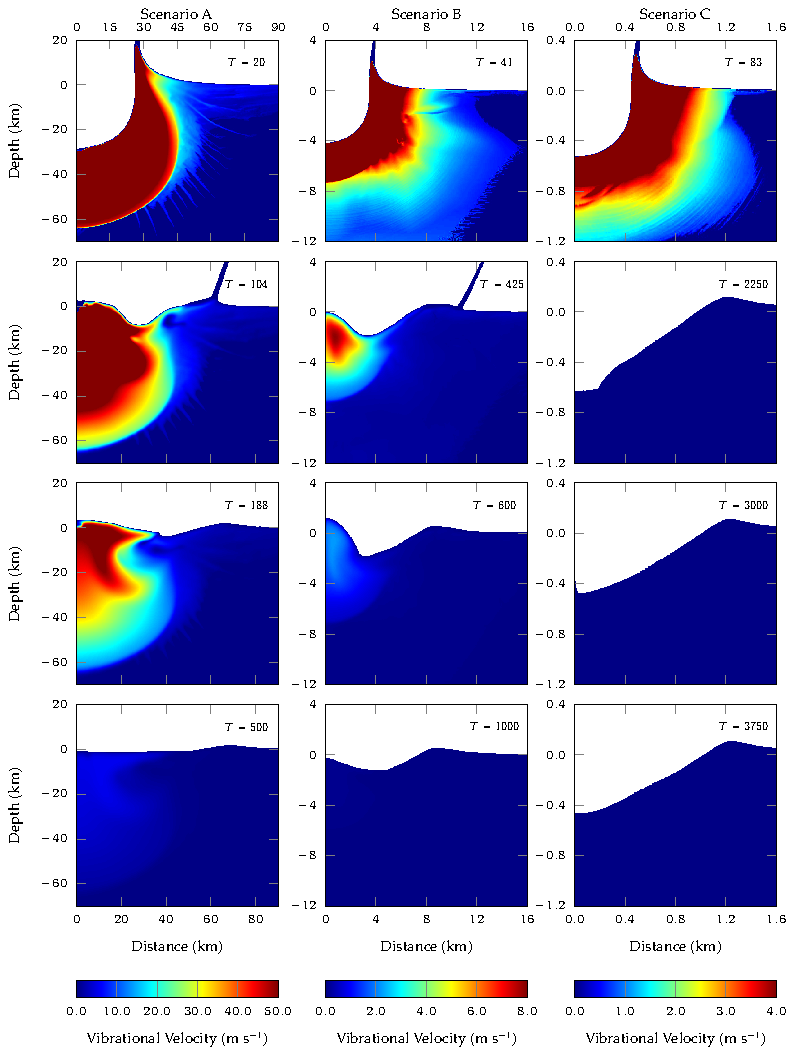
\includegraphics[width=0.7\linewidth]{./images/block_velo.pdf}
\caption{The evolution of acoustic vibrations for the block model in scenarios A, B and C. The zone of intense vibrations decreases in size as vibrations decay after the initial distribution of acoustic energy. This occurs the fastest in scenario C. Decay is strongest laterally in scenarios A and B. Note the different colour scales used here. \label{fig:block_velo}}
\end{figure*}

Crater formation time is greatest for large impacts. Consequently, it is difficult to compare crater formation stages for impacts of different sizes. The approach used here is to non-dimensionalise time using the shock wave propagation time, which is approximately proportional to impactor size divided by velocity. Thus the non-dimensional time $T$ is related to time via:

\begin{equation}
T=\frac{Ut}{a}
\end{equation}

where $U$ is the impactor velocity, $t$ is the simulation time in seconds, and $a$ is the impactor radius \citep{o1993planetary}.

Several non-dimensional time slices showing the evolution of acoustic vibrations for the block and Melosh models are shown in figures \ref{fig:block_velo} and \ref{fig:melosh_velo}, respectively. Scenarios A, B and C are shown from left to right in both figures.

\subsection{Block Model Evolution of Acoustic Vibrations}\label{sec:blockvelo}

\begin{figure*}[!b]
\centering
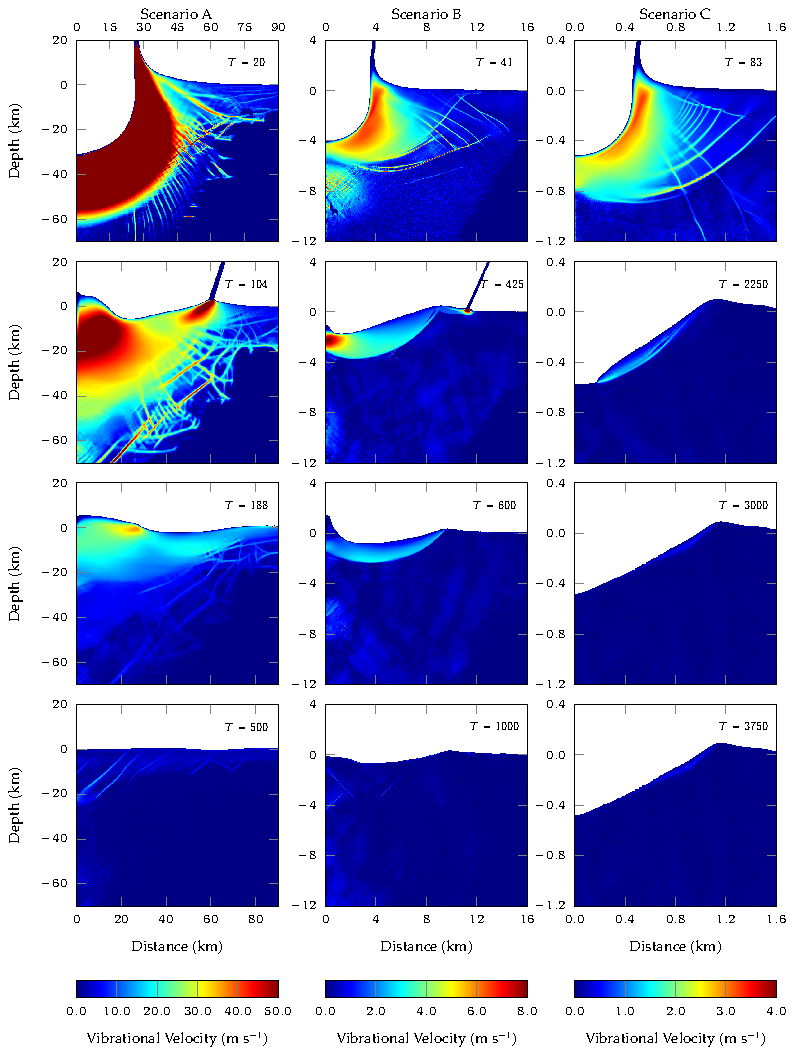
\includegraphics[width=0.7\linewidth]{./images/melosh_velo.pdf}
\caption{The evolution of acoustic vibrations for the Melosh model in scenarios A, B and C. Localised regions of vibrational velocity are evident throughout all scenarios. As in the block model, the rate of acoustic dissipation increases from scenarios A to C, where vibrations dissipate the fastest. Decay is strongest vertically in scenarios A and B. There is also significant regeneration of acoustic vibrations in localised regions of the domain. Note the different colour scales used here. $\lambda=0.2a$ and $Q=10$. \label{fig:melosh_velo}}
\end{figure*}

\begin{figure*}[!t]
\centering
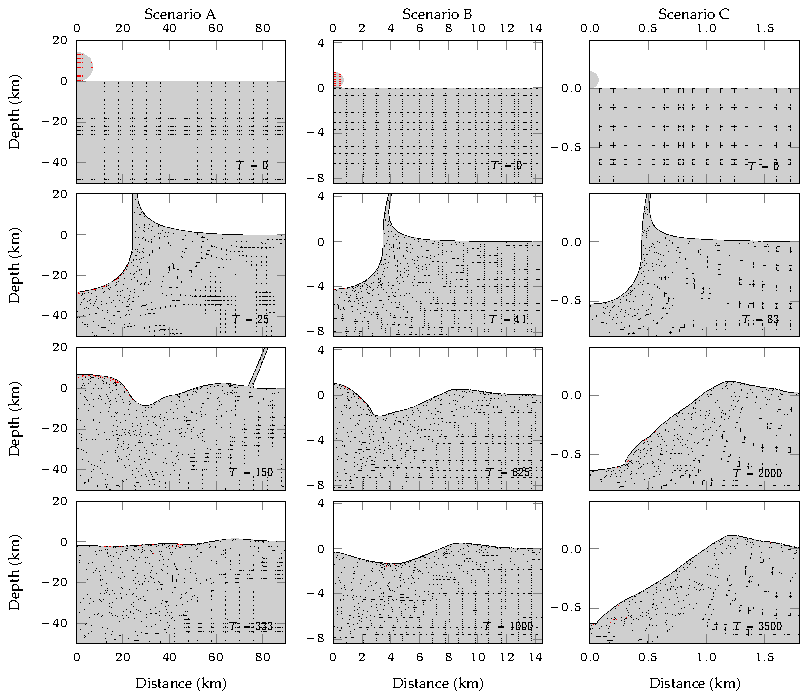
\includegraphics[width=0.99\linewidth]{./images/block_deformation.pdf}
\caption{Evolution of subcrater deformation in the block model for scenarios A, B and C. The style of deformation is much the same for the second time slice across all scenarios. Scenarios A and B both show large central uplifts in the third time slice, while the bottom of the transient crater in scenario C does not rebound at all. All scenarios show inward rim collapse in the third time slice. \label{fig:block_deformation}}
\end{figure*}


\begin{figure*}[!t]
\centering
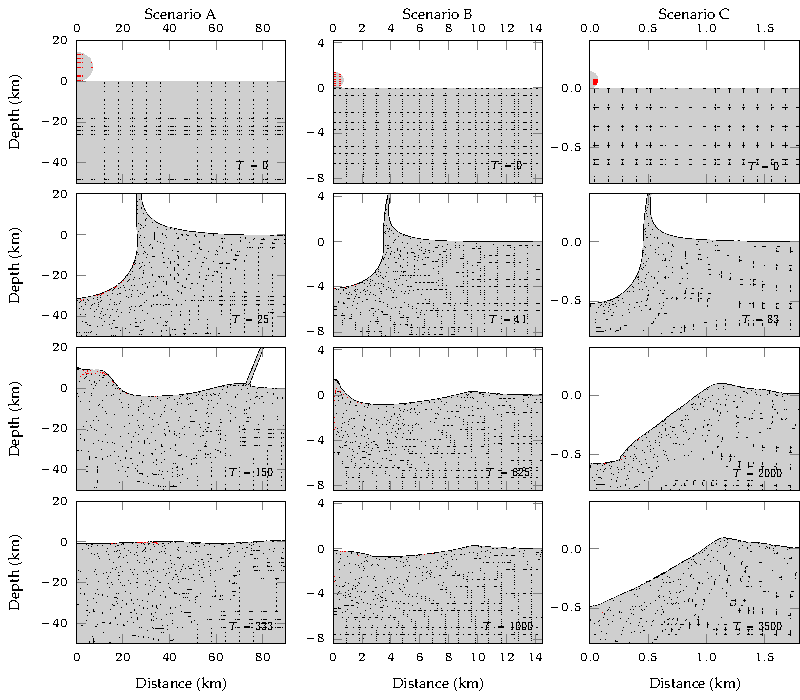
\includegraphics[width=0.99\linewidth]{./images/melosh_deformation.pdf}
\caption{Evolution of subcrater deformation in the Melosh model for scenarios A, B and C. As in the block model, the style of deformation is very similar for all three scenarios at the second time slice. Scenario A  has a much wider central uplift than B in the third time slice. All scenarios show inward rim collapse in the third time slice. $\lambda=0.2a$ and $Q=10$. \label{fig:melosh_deformation}}
\end{figure*}



%\newgeometry{top=1.5cm,bottom=2cm,left=4cm,right=2.5cm}

\begin{figure*}[!t]
\centering
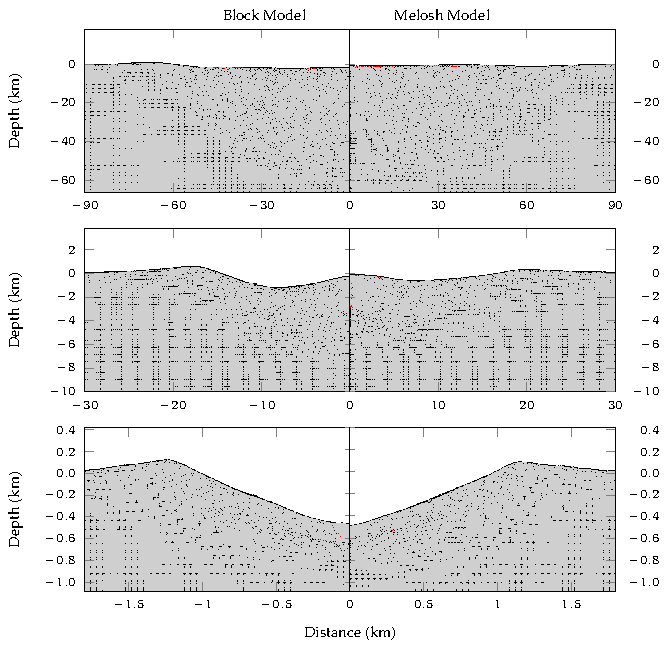
\includegraphics[width=0.8\linewidth]{./images/comparison.pdf}
\caption{A comparison of all final crater morphologies using the block (left) and Melosh (right) models of acoustic fluidisation for scenarios A (top), B (middle) and C (bottom). Both models produce similar crater morphologies for their respecitve scenarios; a peak ring complex crater in scenario A, a central peak crater in scenario B, and a simple crater in scenario C. $\lambda=0.2a$ and $Q=10$ for the Melosh model. \label{fig:comparison}}
\end{figure*}

\begin{figure*}[!t]
\centering
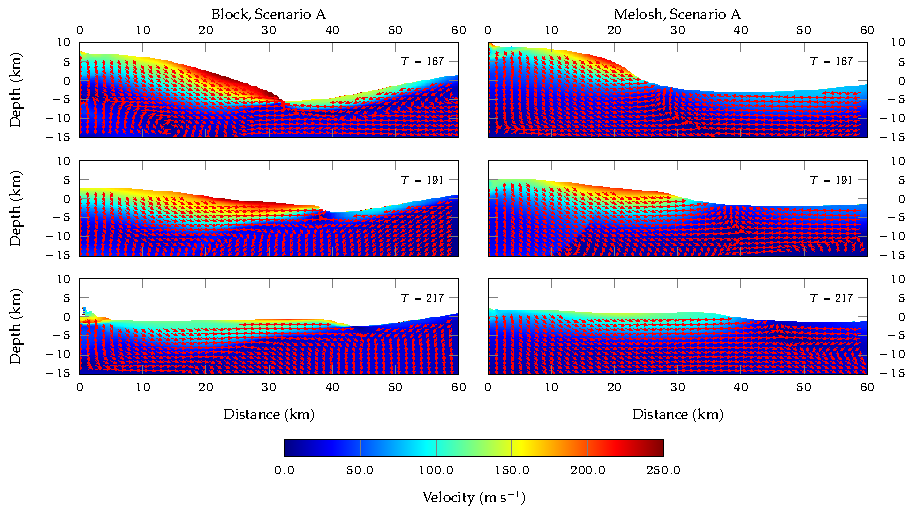
\includegraphics[width=\linewidth]{./images/peak_ring.pdf}
\caption{A comparison of velocity vectors during peak ring formation between the block and Melosh models for scenario A. It is evident that rock material is forced under the outwardly collapsing inner material for the block model. In the Melosh model, however, inwardly collapsing material is forced up against the outardly collapsing material, forming a central peak at the confluence between the two. $\lambda=0.2a$ (7200m) and $Q=10$.\label{fig:peak_ring}}
\end{figure*}

The broad, spatial characteristics of the initial vibrational velocity field for all scenarios in the block model (Figure \ref{fig:block_velo}) show deep zones of intense acoustic vibrations ($v_{vib} > 50$ m s$^{-1}$). At no point in any scenario are vibrations focused or localised into any region of the domain. After the shock wave has passed in the second and third time slices, the zone of intense vibrations  begins to decay, shrinking in size. In scenario A, the strongest decay occurs laterally, causing intense vibrations to persist at depth in the third time slice. Strong lateral decay in scenario B also reduces intense vibrations into a small area centred directly inside the central uplift, as in scenario A. Decay occurs the fastest in the smallest scenario, C. 

Intense acoustic vibrations are not evident at the edge of the crater during the second and third time slices in any scenario. This is particularly important in scenarios A and B, which require a collapsed rim to form a complex crater.

Crater formation ends in the fourth time slice, when all vibrations have ceased.

\subsection{Melosh Model Evolution of Acoustic Vibrations}\label{sec:meloshvelo}

In some respects, the initial, broad, spatial variation in vibrational velocity in the Melosh model in Figure \ref{fig:melosh_velo} is much like that of the block model, particularly for scenario A. Again, intense vibrations extend deep into the target, although the magnitude of the vibrational velocity in scenarios B and C is much less than that in the block model. The most important difference, however, is the presence of localised vibrations in all scenarios of the Melosh model. 

In the second time slice, the size of the zone of intense vibrations decays faster than in the block model, and as a result is smaller in size. In contrast to the block model, decay occurs primarily in the vertical direction. A significant number of localised vibrations are also regenerated near the surface, particularly around the crater rim and central uplift in scenarios A and B.

There are significant acoustic vibrations laterally in the third time slice for the largest two scenarios, with vibrations spanning from the crater center to the crater rim. As in the block model, vibrations decay the fastest for scenario C.

\subsection{Subcrater Deformation \label{subsec:comparison}}

Figures \ref{fig:block_deformation} and \ref{fig:melosh_deformation} show the evolution of subcrater deformation in a series of time slices for the block and Melosh models, respectively. The dashed lines represent tracer particles, tracking the movement of rock material from its pre-impact position. The first time slice shows the initial condition of each model - the point at which contact and compression begins. The second time slice, taken during excavation, shows little difference in subcrater deformation in all scenarios, for both the block and Melosh models alike.

However, a range of differences in subcrater deformation arise in the third time slice, during modification. In scenario A, both models form a large central uplift. Radially, the block model's central uplift is around 10km larger than the Melosh uplift.

In scenario B, at time slice $T=625$, both models again form a large central uplift. Material existing just outside of the uplift core is primarily that which is uplifted into the developing central peak for the Melosh model. This contrasts with the block model, where central uplift material mostly originates from directly below the point of impact. As in scenario A, the central uplift is largest in the block model by $\sim$ 3km.

There is very little difference between the Melosh and block models in the final two time slices of scenario C. Both show displaced material collapsing back into the centre of the crater, forming a steep sided simple crater. 

A comparison of final crater morphology and subcrater deformation between the two models is shown in Figure \ref{fig:comparison}. Again, there is little difference between the two models in scenario C. The Melosh model produces a shallower crater in scenario B, and it is also evident that the vertical extent of subcrater deformation is smaller  than in the block model. This is especially true in scenario A.

The differing particle velocity fields for both models during peak ring formation in scenario A suggest two different modes of peak ring formation (Figure \ref{fig:peak_ring}). In the block model, central rock material collapses outwards on top of the inwardly collapsing rim. However, in the Melosh model, inwardly collapsing material is forced up against the outwardly collapsing material.
